
%!TEX root = Main.tex
\documentclass[Main]{subfiles}

\begin{document}

\section{Robot Mechanics} % (fold)
	\label{sec:robot_mechanics}

	\subsection{Chassis} % (fold)
		\label{sub:chassis}
The chassis of the robot is a Baron-4WD mobile platform bought from the website dfrobots.com. 
It consist of a lower frame where up to four DC motors can be attached, and a top plate with holes for mounting of other devices. 
\autoref{fig:baron_platform} shows a picture of the chassis where it is assembled with the default package items from dfrobots.
\begin{figure}[H]
	\centering
	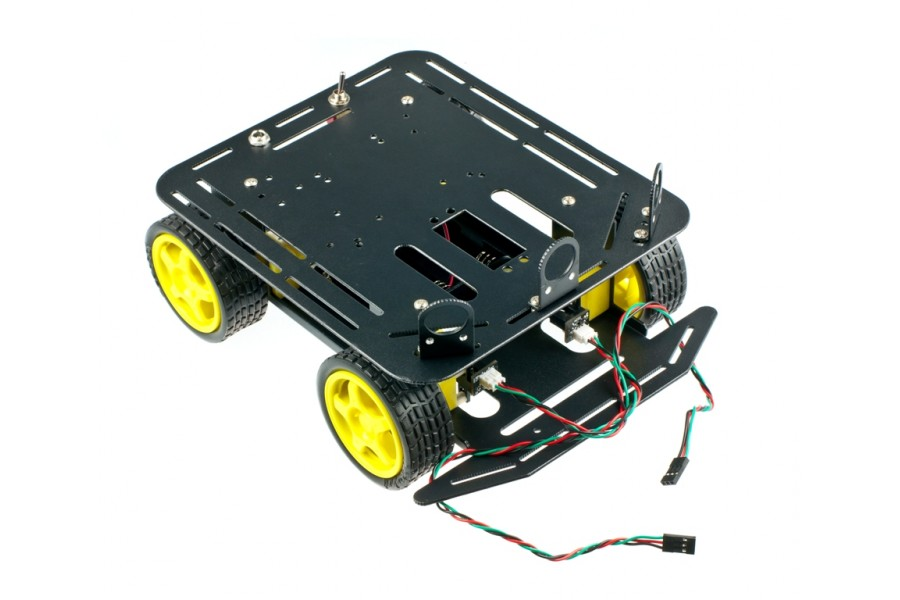
\includegraphics[width=0.5\linewidth]{./Figures/baron_platform.jpg}
	\caption{The Baron-4WD platform}
	\label{fig:baron_platform}
\end{figure}\noindent
In this project it was decide to only use two motors at the rear end of the chassis to make a simpler motion model for the robot; more about the motion model in \autoref{sub:motion_model}. 
Instead of front wheels, a ball caster was attach to insure the turning ability. 
By only using motors in the rear end, the lower frame had a lot of room where the power supplies could be place and thereby leaving the top plate free for the processing platform, a Zybo development board \fxnote{ref}, and mounting of the sensors. 
The sensor used in this project was a LIDAR \fxnote{ref} which required a specific mounting pattern, that filled out most of the top plate's area, thereby only leaving a small area for the Zybo board. 
The LIDAR was therefore mounted on a acrylic plate which then was mounted on top of the top plate. 
The final robot configuration is shown in \autoref{fig:final_robot}.
\begin{figure}[H]
	\centering
	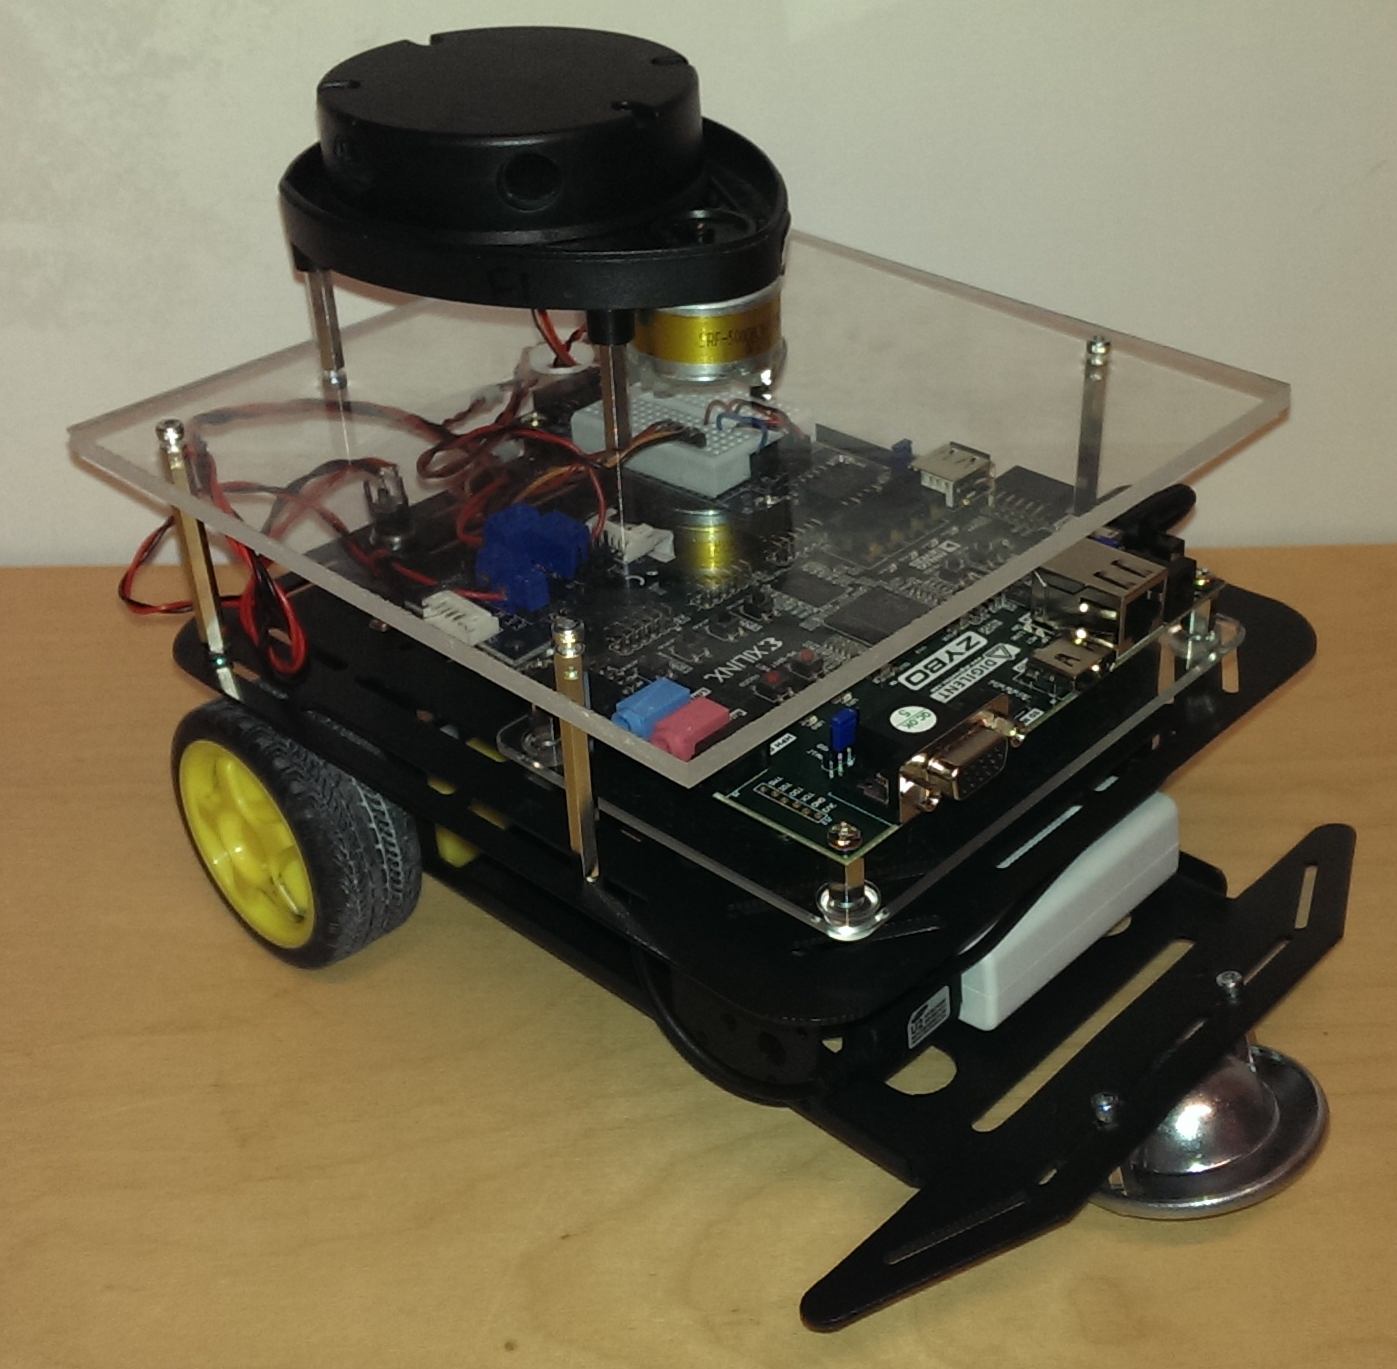
\includegraphics[width=0.5\linewidth]{./Figures/final_robot.png}
	\caption{The final robot configuration}
	\label{fig:final_robot}
\end{figure}\noindent
		% subsection chassis (end)

	\subsection{Motor characteristics} % (fold)
		\label{sub:motor_characteristics}
		
		% subsection propulsion (end)

	\subsection{Motion model} % (fold)
		\label{sub:motion_model}
The motion model used in this project is based on a simple rotation and the move model.
The rotation is however not just a change in orientation since the robot is not rotating around it's center of mass.
When rotating, the robot is rotating around one of it's wheel which means that the center of mass is also being move during this.
The difference between these to rotations are shown in
\begin{figure}
\begin{subfigure}
\centering
	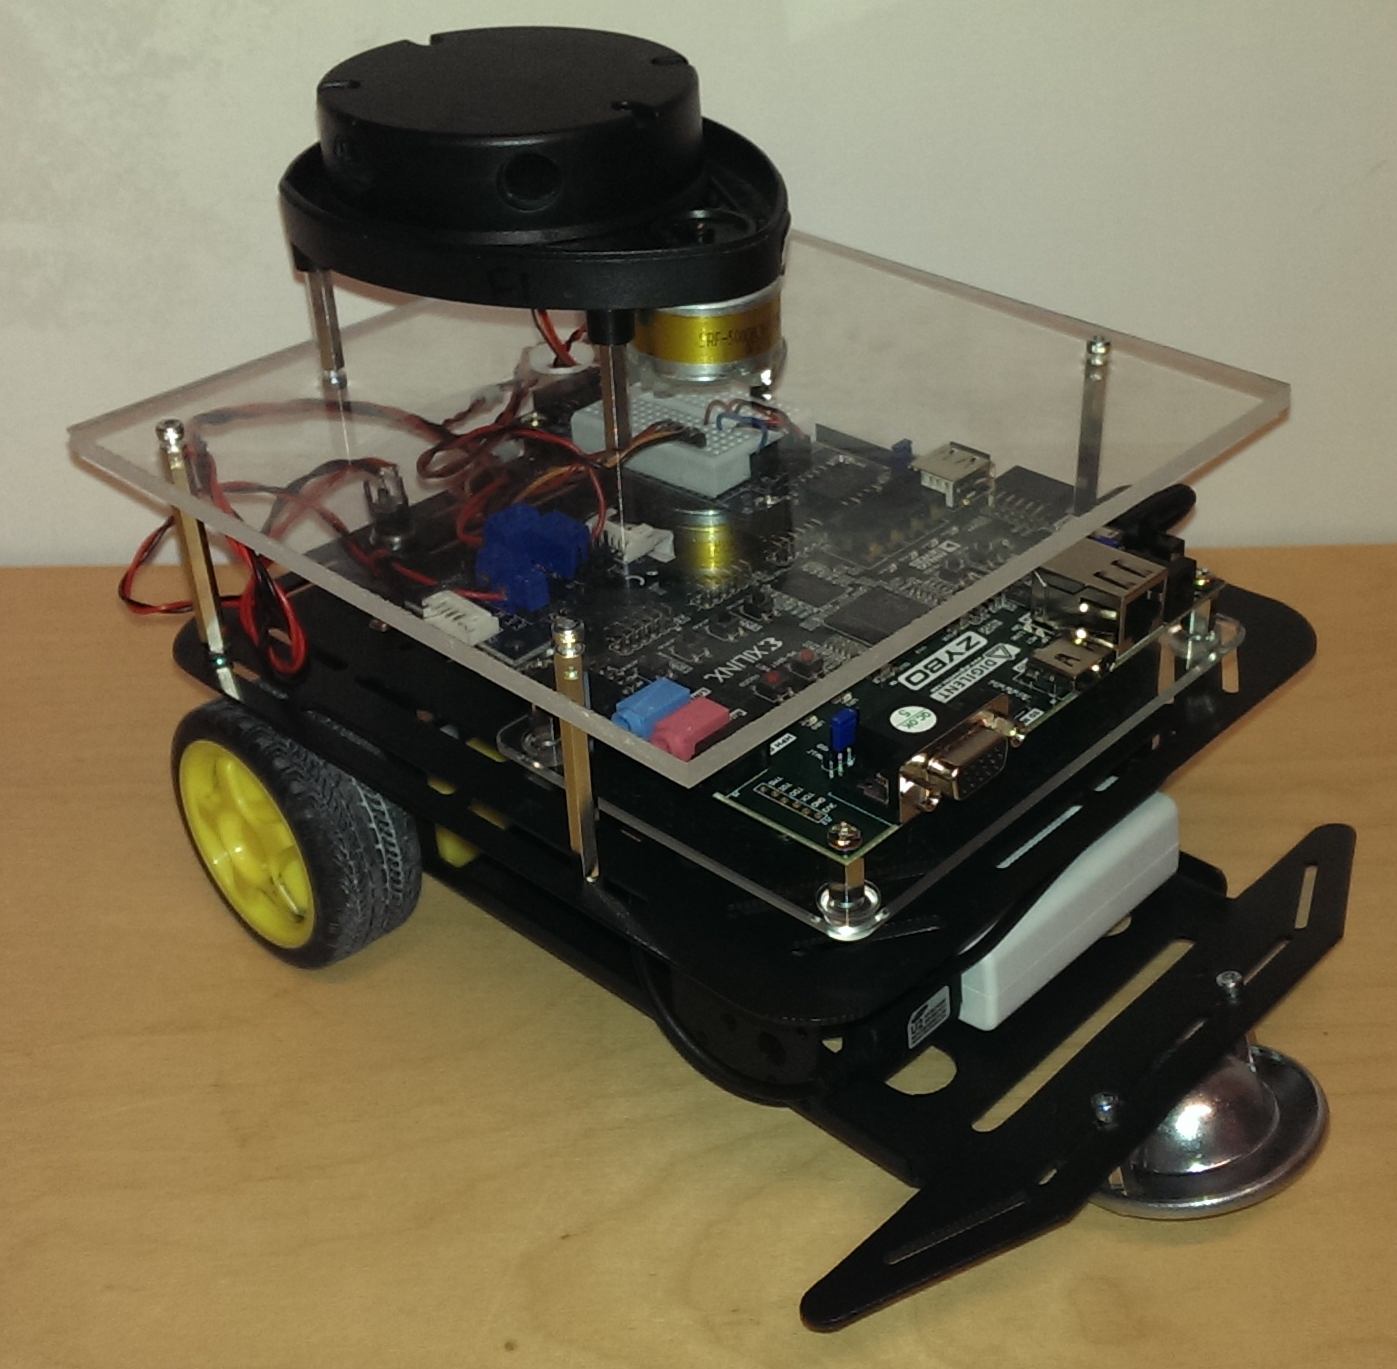
\includegraphics[scale=1]{./Figures/final_robot.png}
	\caption{The final robot configuration}
	\label{fig:final_robot}
\end{subfigure}
\begin{subfigure}
\centering
	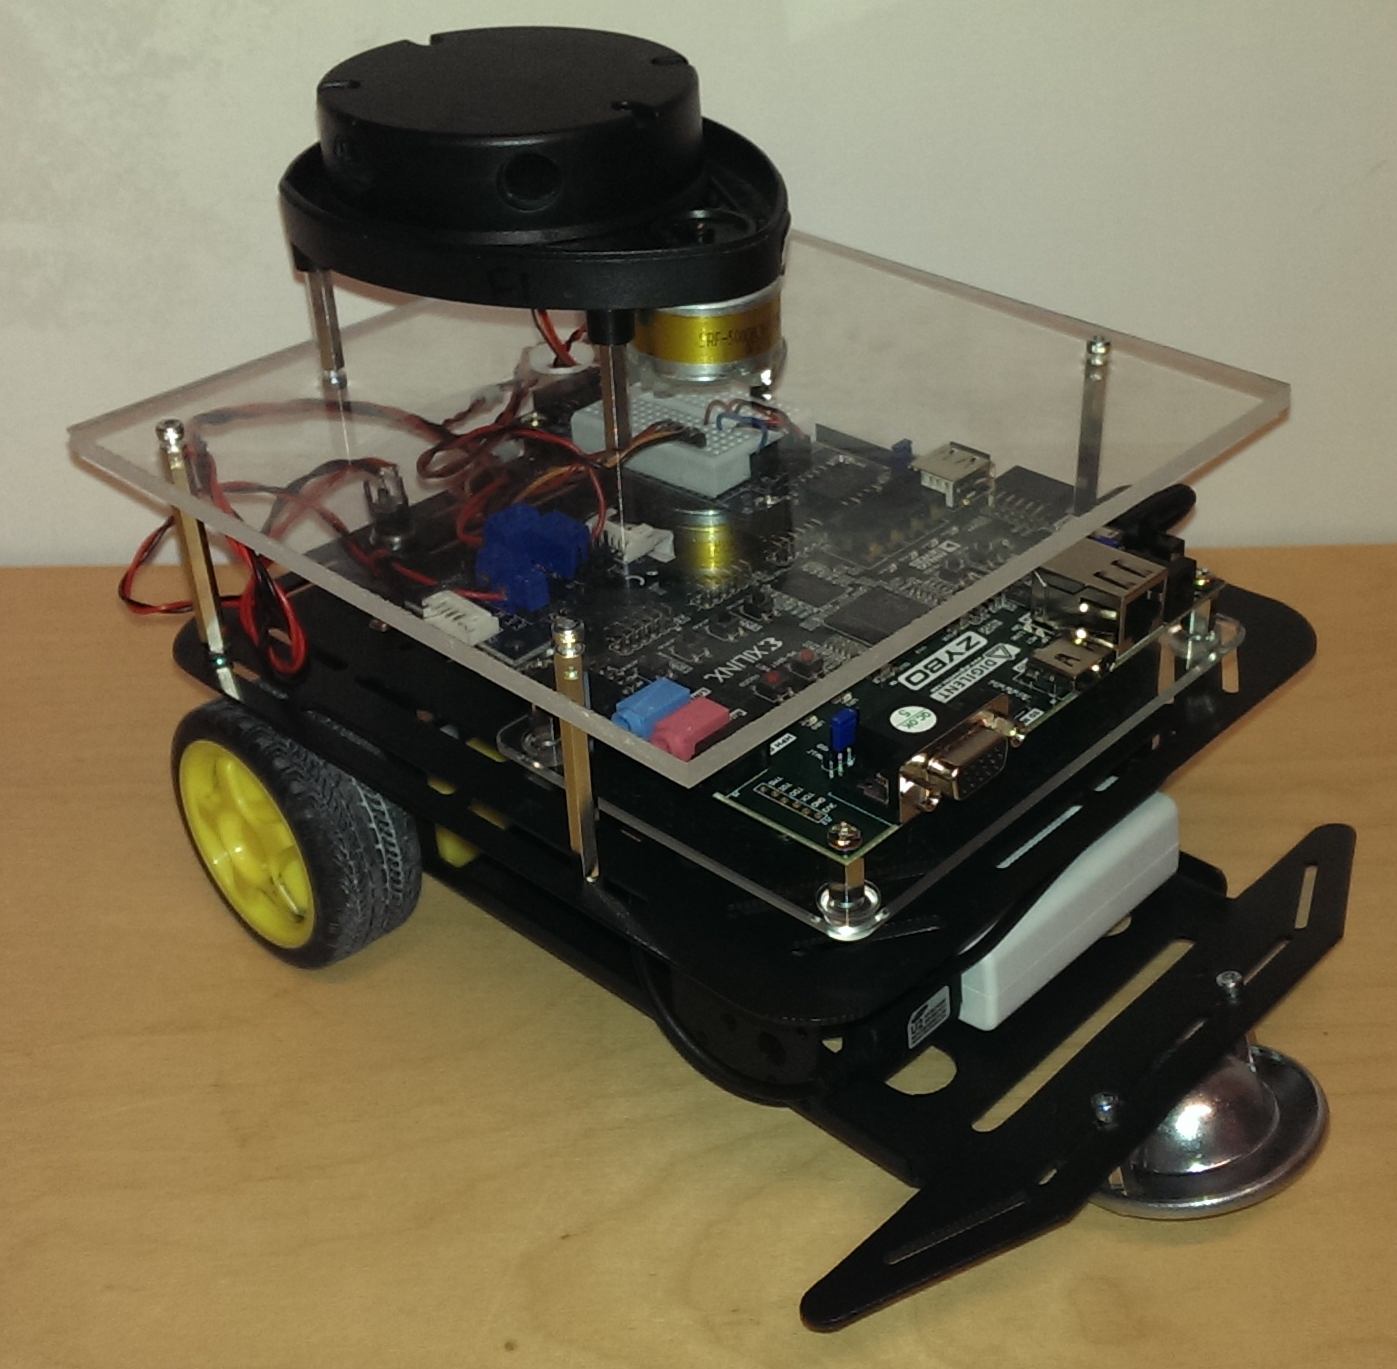
\includegraphics[width=0.5\linewidth]{./Figures/final_robot.png}
	\caption{The final robot configuration}
	\label{fig:final_robot}
\end{subfigure}
\caption{The final robot configuration}
\label{fig:final_robot}
\end{figure}

		% subsection motion_model (end)

	% subsection robot_mechanics (end)

\end{document}